\section{Intel FPGA Overview}
Im Kurs wird ein MSE-Embedded Board als Labor-Hardware. Dieses basiert auf einem Intel FPGA, desseb Eigenschaften und Eigenheiten im nachfolgenden Kapitel beschrieben ist
\subsection{Cyclon IV}
Das MSE-Embedded Board ist mit einem Intel Cyclon IV FPGA vom Typ EP4CE30 bestückt. Das Datenblatt spezifiziert dabei folgendes:

\newcolumntype{C}[1]{>{\centering\let\newline\\\arraybackslash\hspace{0pt}}m{#1}}
\newcolumntype{L}[1]{>{\let\newline\\\arraybackslash\hspace{0pt}}m{#1}}
\begin{table}[h!]
\begin{center}
 \begin{tabular}{|p{8cm}|| C{4cm}|} 
 \hline
 \textbf{Logic Elements} & 28'848 \\
 \hline
 \textbf{9K memory blocks} & 66	\\
 \hline
\textbf{Embedded memory (Kb)} & 594\\
 \hline
\textbf{18-bit x 18-bit multipliers} & 66\\
 \hline
\textbf{PLLs} &4\\
 \hline
\textbf{Maximum user I/Os} & 532\\
 \hline
\textbf{Maximum differential channels} & 52\\
 \hline
  \end{tabular}
 \caption{Technische Daten EP4CE30}
\end{center}
\end{table}

\subsubsection{Logic Element}
Intel Altera versteht unter einem Logic Element (LE) ein Block mit dem folgenden Aufbau:
\begin{figure}[h!]
\centering
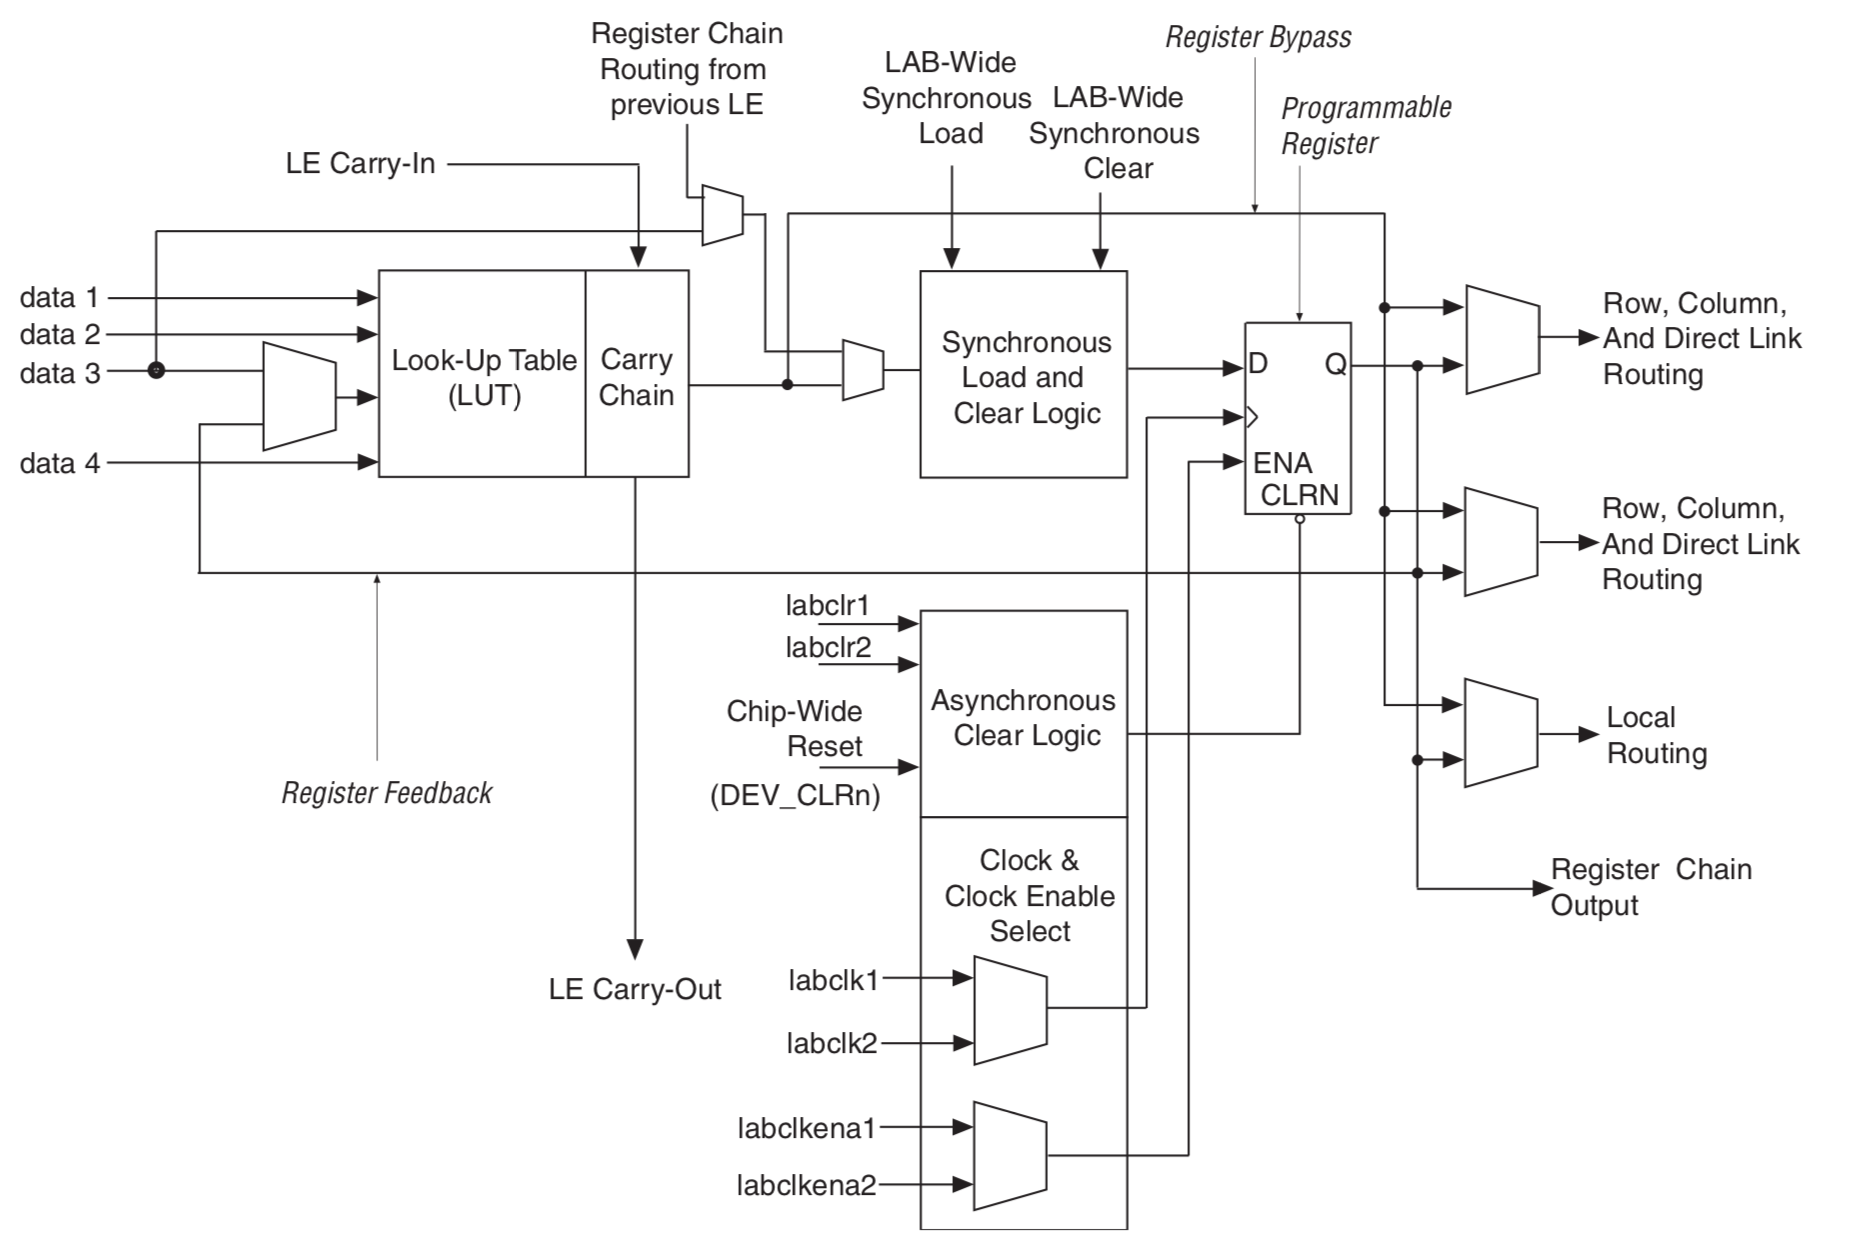
\includegraphics[width=13cm]{pic/logicelement.png}
\caption{Altera Logic Element}
\end{figure}

Jedes Logic Element kann als D-, T-, JK- oder SR-Flip-Flop konfiguriert werden. Zudem besitzt jedes Register eine Data, Clock, Clock Enable und eine Clear Input-Leitung. \\
Das Logic Element kann in zwei verschiedenen Modi betrieben werden, entweder im ''Normal-Mode'' im ''Arithmetic-Mode''. Während im Normal Mode das Carry-In als normalen Daten-Input einer 4-LUT benutzt wird, wird die LUT im Arithmetic Mode zu einem Full-Adder (mit Carry) konfiguriert. 
\subsubsection{Logic Array Block}
Ein Logic Array Block gruppiert Logic Elements. Jedes LAB besteht aus den folgenden Teilen
\begin{itemize}
\item 16 Logic Elements (LEs)
\item LAB Control Signals
\item LE Carry Chain
\item Register Chain
\item Local Interconnect
\end{itemize}
Der Local Interconnect transportiert Signale zwischen dem Logic Element und dem LAB. Register Chains verbinden angrenzende Flip-Flops miteinander. 
\subsection{Nios-II}
Im Modul wird ein soft-core Prozessor vom Typ Nios II verwendet. Nios-II ist eine synthetisierbare 32-Bit RISC CPU in Harvard Architektur, vergleichbar mit Xilinx MicroBlaze. Im Unterschied zu MikroBlaze ist diese aber lizenzierbar für die Verwendung in einem ASIC. Es stehen dem User zusätzlich 256 freie Instruktionen zur Verfügung, die bei der synthese in die ALU integriert werden. Dies erlabut es applikationsspezifische Instruktionen zu erstellen. Zudem werden Betriebssysteme wie Linux, eCos, embOS, Euros RTOS, oSCAN, uCLinux, ThreadX oder VxWorks unterstützt. Den Nios II wird durch drei verschiedene Ausführungsvarianten der Anwendung angepasst werden. Entsprechend muss zwischen Speed vs. Area vs. Power entschieden werden.
\begin{table}[h!]
\begin{center}
\begin{tabular}{l|l|l|l}
 & Nios II/f & Nios II/s & NiosII/e \\
 \hline
 \textbf{Type} & fast & standard & economy \\
 \textbf{Pipeline} & 6 stages & 5 stages & none\\
 \textbf{Branch prediction} & dynamic & static &none\\
 \textbf{Inst Cache} & configurable & configurable & none\\
 \textbf{Data Cache} & configurable & none & none\\
 \textbf{MMU} & Yes & No & No\\
 \textbf{HW Multiplier} &1 cycle & 3 cycle & none\\
 \textbf{HW Divider} & Yes & Yes & no\\
 \textbf{Resources} & $\approx$ 2'500LEs & $<$ 1'400LEs & $<$ 700LEs \\
 \textbf{Maximum frequency} & 290 MHz & 270 MHz & 340 MHz\\
\end{tabular}
\caption{Verschiedene Nios-II Konfigurationen}
\end{center}
\end{table}
\subsubsection{Custom Instructions}
Dem Nios II stehen 256 Selektoren für Custom Instructions (CI) zur Verfügung. Es können sowohl rein kombinatorische Instruktionen wie auch Multicycle Instructions erstellt werden. Die Custom Logik wird parallel zur ALU synthetisiert und mit derer Ausgangs-MUX verbunden.
\newpage
\begin{figure}[ht!]
\centering
\savebox{\largestimage}{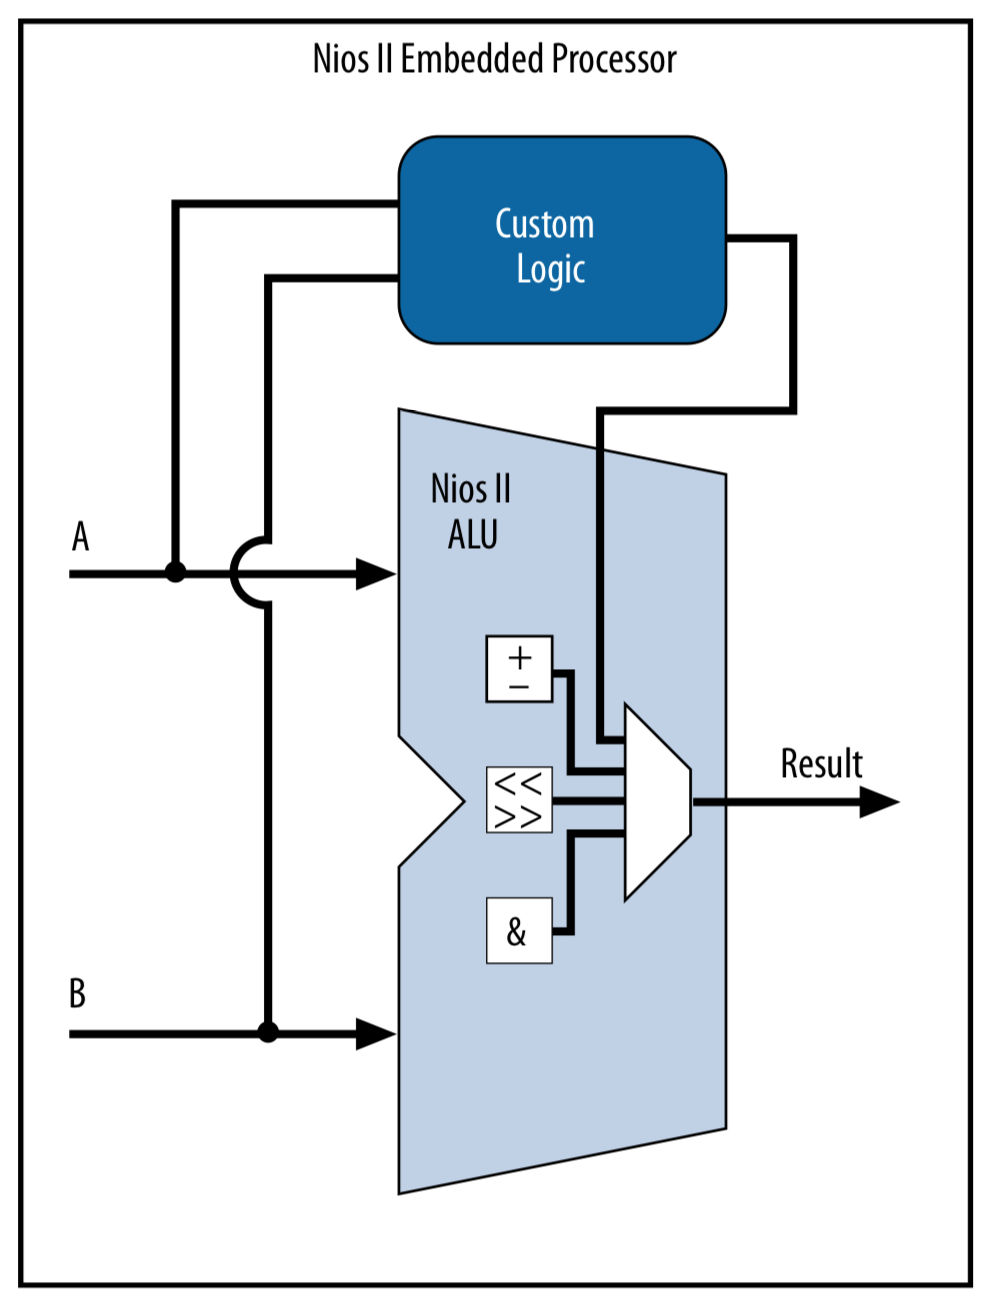
\includegraphics[height=.3\textheight]{pic/custom_instruction.png}}
\begin{subfigure}[b]{0.4\textwidth}
    \centering
    \usebox{\largestimage}
\caption{Blockdiagramm  der CI}
 \end{subfigure}
 \begin{subfigure}[b]{0.4\textwidth}
 \centering
    % Adjust vertical height of smaller image
    \raisebox{\dimexpr.5\ht\largestimage-.5\height}{%
      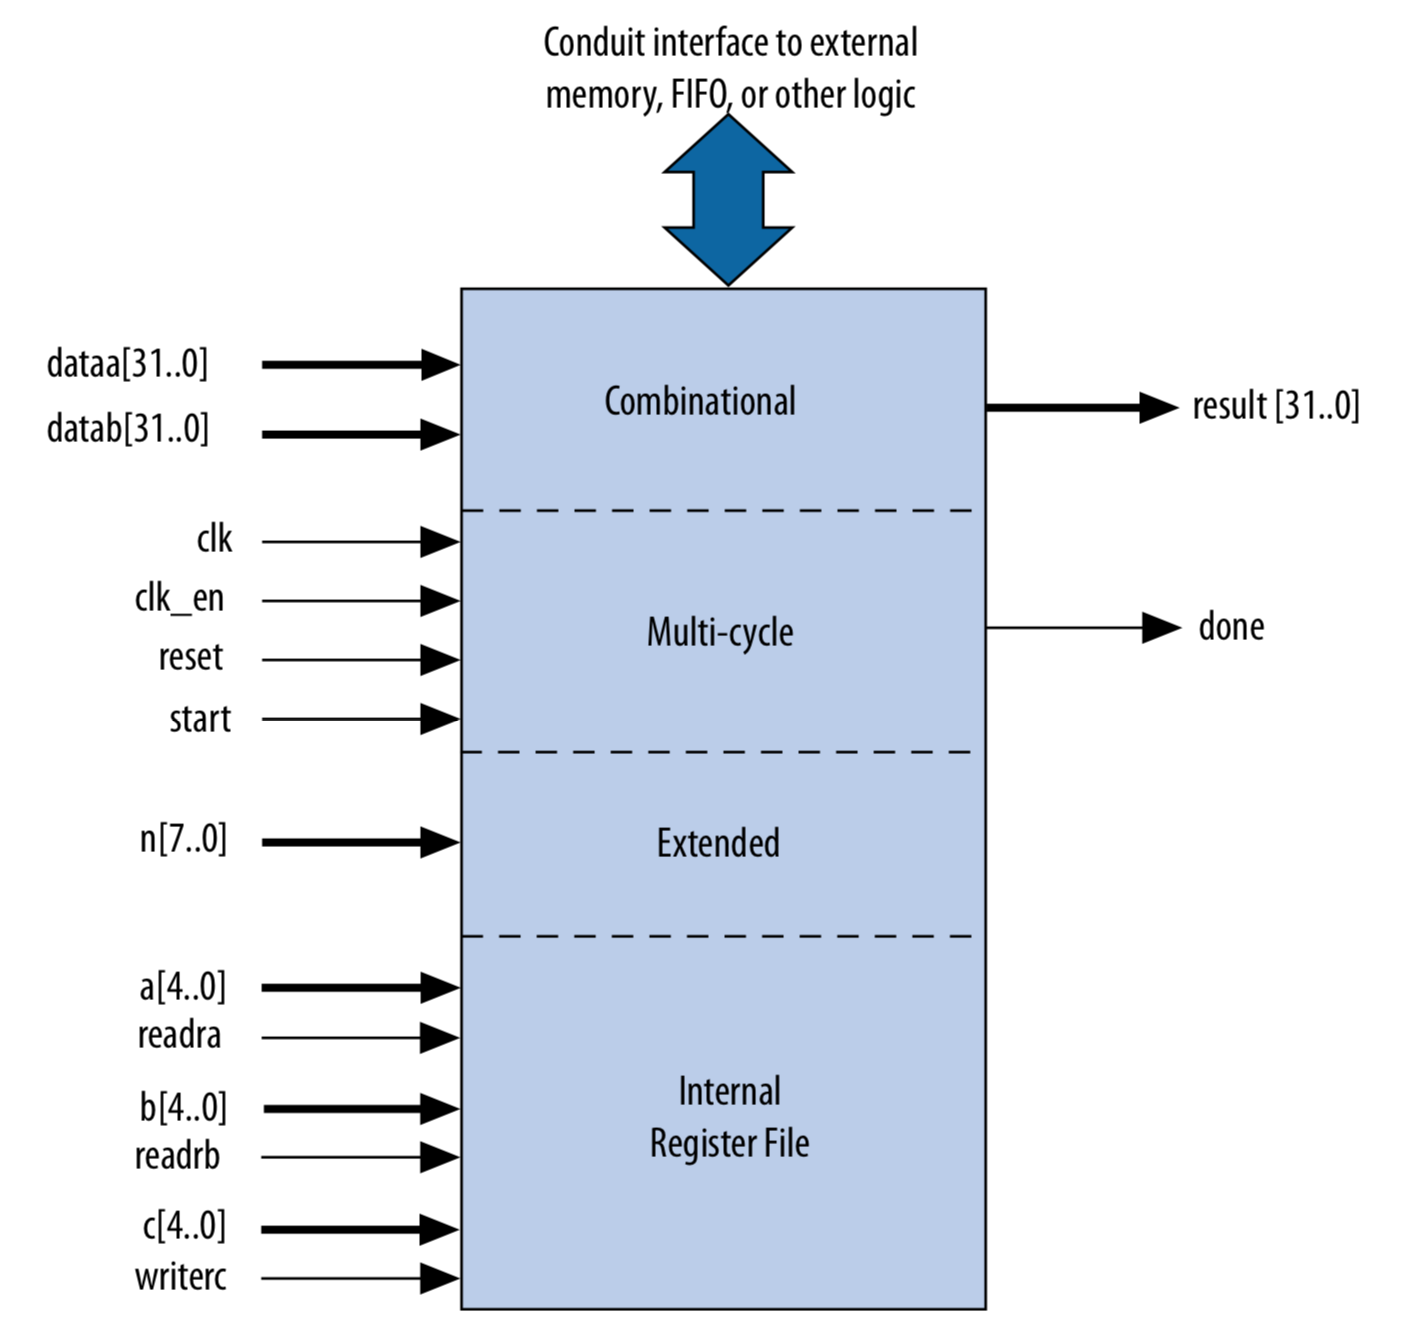
\includegraphics[height=.3\textheight]{pic/custom_instruction_signals.png}}
\caption{benötigte Nios-II Signale}
 \end{subfigure}
 \caption{Prinzip einer Custom Instruction}
\end{figure}
Die beiden Abbildung zeigen, welche Signale für unterschieldiche Typen von CI benötigt werden. 
Während für eine rein kombinatorische Instruktion nur die \code{dataa} und \code{datab} benötigt werden, sind für Multi-Cycle Instruktionen auch \code{clk}, \code{clk\_en}, \code{reset}, \code{start}-Eingänge und ein \code{done}-Ausgang gefordert. Der Extended-Modus erlaubt es, innerhalb einer CI verschiedene Operationen durchzuführen, welche mit dem \code{n[7..0]}-Vektor selektiert wird. Mit einer Internal Register-File-Instruktion kann auf interne Register zugegriffen werden. (als Input oder Output)
\subsubsection{Interrupt Controller}
Der Nios-II hat 32 interne Hardware Interrupts wovon jeder Interrupt seinen eigenen Interruptvektor besitzt. \code{[irq0..irq31]} Die Interruptpriorität wird durch die Software gesetzt. Weiter hat der Interruptcontroller folgende Funktionalitäten:
\begin{itemize}
\item \code{isenabled}-Flag ermöglicht individuelle aktivierung/deaktivierung
\item \code{PIE}-Flag ermöglicht globale aktivierung/deaktivierung
\end{itemize}
Die folgenden Commands entstammen der API und bilden die grundsätzlichen Softwarezugriffe auf die Interrupt-Hardware:
\begin{table}[h]
\begin{tabular}[t]{p{.2\textwidth} p{.7\textwidth} }
Prototype & \lstinline$int alt_irq_register(alt_u32 id, void* context, $ \\
& \lstinline$void (*isr)(void*, alt_u32)$  \\
Description & The \lstinline$alt_irq_register()$ function registers an ISR. If the function is successful, the requested interrupt is enabled on return. \lstinline$context$ and \lstinline$id$ are the two input arguments to isr.\\
Arguments & \lstinline$alt_u32 id$:	ISR ID \\
 & \lstinline$void* context$: 	Pointer to context argument for ISR\\
 & \lstinline$void (*isr)(void*, alt_u32)$ : Function Pointer to ISR\\
Return &  zero if successful, non-zero otherwise. 
\end{tabular}
\end{table}
\begin{table}[h!]
\begin{tabular}[t]{p{.2\textwidth} p{.7\textwidth} }
Prototype & \lstinline$int alt_irq_enable(alt_u32 id)$ \\
Description & The \lstinline$alt_irq_enable()$ function enables a single interrupt\\
Arguments & \lstinline$alt_u32 id$:	ISR ID \\
Return &  zero
\end{tabular}
\end{table}
\begin{table}[h!]
\begin{tabular}[t]{p{.2\textwidth} p{.7\textwidth} }
Prototype & \lstinline$int alt_irq_disable(alt_u32 id)$ \\
Description & The \lstinline$alt_irq_disable()$ function disables a single interrupt\\
Arguments & \lstinline$alt_u32 id$:	ISR ID \\
Return &  zero
\end{tabular}
\end{table}
\begin{table}[h!]
\begin{tabular}[t]{p{.2\textwidth} p{.7\textwidth} }
Prototype & \lstinline$alt_irq_context alt_irq_disable_all(void)$ \\
Description & The \lstinline$alt_irq_disable_all()$ disables all maskable interrupts. Nonmaskable interrupts (NMIs) are unaffected.\\
Arguments & none \\
Return &  Pass the return value as the input argument to a subsequent call to \lstinline$alt_irq_enable_all()$.
\end{tabular}
\end{table}
\begin{table}[h!]
\begin{tabular}[t]{p{.2\textwidth} p{.7\textwidth} }
Prototype & \lstinline$void alt_irq_enable_all (alt_irq_context context)$ \\
Description & The \lstinline$alt_irq_enable_all()$ function enables all interrupts that were previously disabled by \lstinline$alt_irq_disable_all()$. The input argument, context, is the value returned by a previous call to \lstinline$alt_irq_disable_all()$. Using context allows nested calls to \lstinline$alt_irq_disable_all()$ and \lstinline$alt_irq_enable_all()$. As a result, \lstinline$alt_irq_enable_all()$ does not necessarily enable all interrupts, such as interrupts explicitly disabled by \lstinline$alt_irq_disable()$.\\
Arguments & \lstinline$alt_irq_context context$  previous interrupt context, returned by \lstinline$alt_irq_disable_all()$.\\
Return &  zero.
\end{tabular}
\end{table}
\newpage
\subsection{Avalon Bus}
Der Avalon Bus ist der Altera-Eigene Kommunikationsbus der Systemkomponenten. Durch den Bus-Standard ist es möglich eigene in Hardware beschriebene Peripherie in die Nios-II Umgebung einzubinden. Die Peripherie kann sowohl Master als auch Slave sein. 
\begin{figure}[h!]
\centering
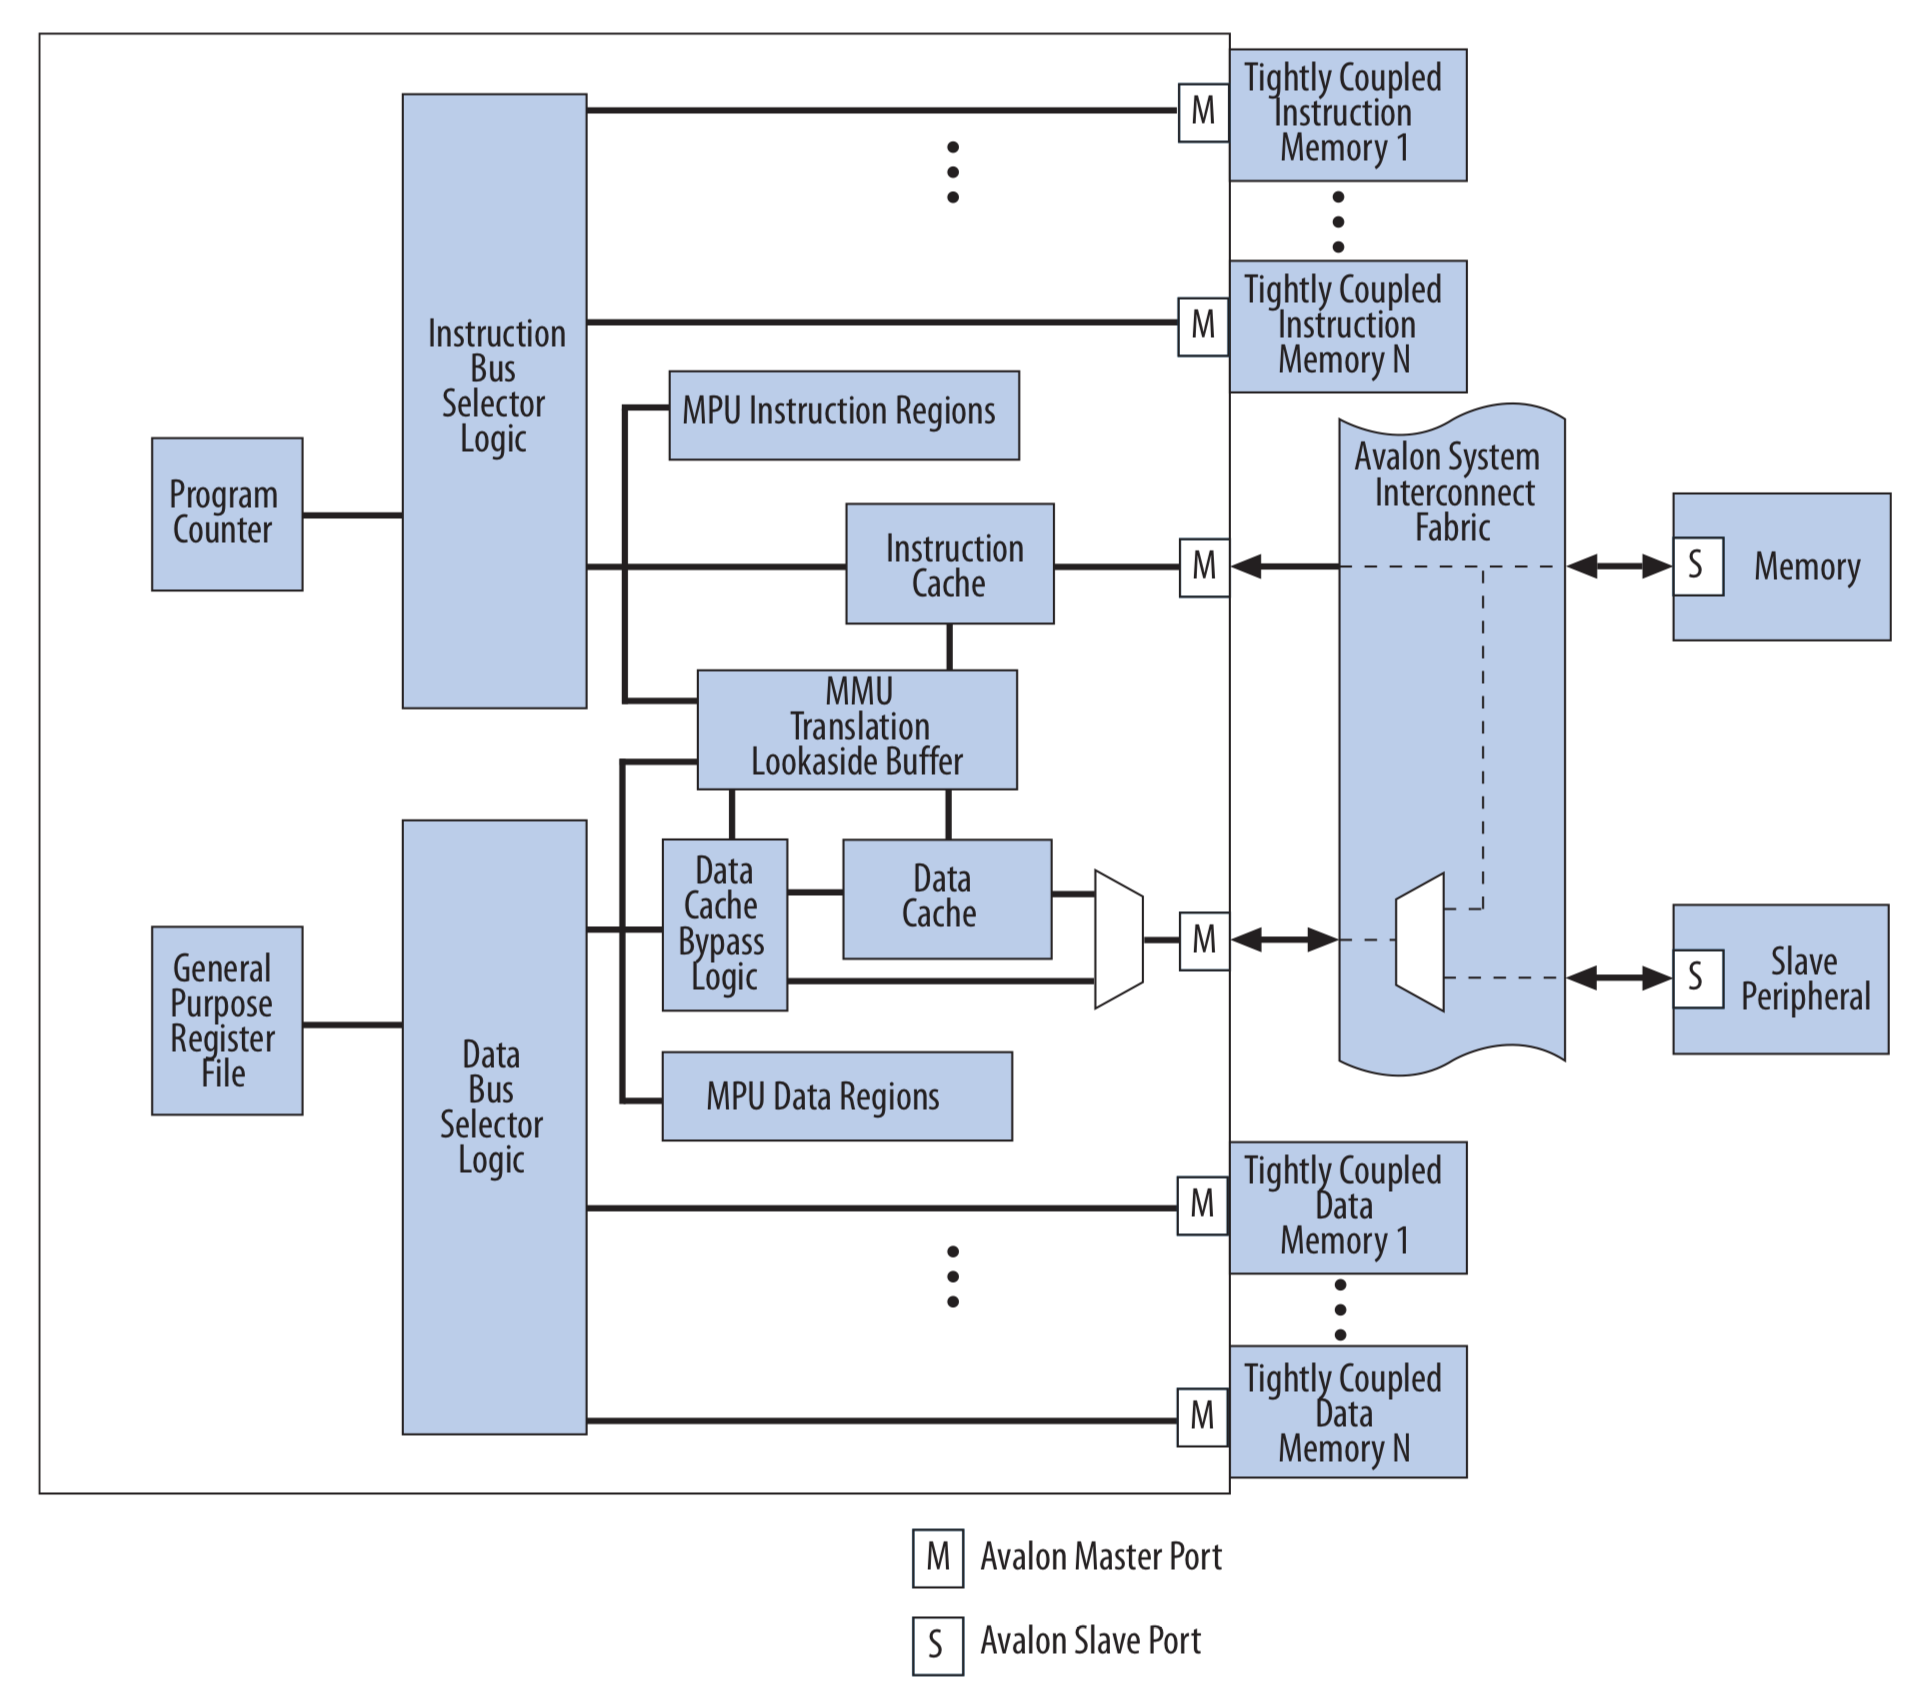
\includegraphics[width=0.5\textwidth]{pic/NiosII_Memory_IO.png}
\caption{Nios-II Memory und I/O Organisation}
\end{figure}
\subsubsection{Avalon Memory-Mapped Interfaces}
Avalon Memory-Mapped (Avalon-MM) interfaces implementieren das Lesen und Schreiben der Master- oder Slave-Komponenten. Folgende Beispiele könnten ein Avalon-MM Interface besitzen
\begin{itemize}
\item Mikroprozessoren 
\item Mermory
\item UART
\item DMA
\item Timers
\end{itemize}






\end{document}


